\documentclass{article}
\usepackage[utf8]{inputenc}
\usepackage{url}
\usepackage{amsmath}
\usepackage{gensymb}
\usepackage{multirow}
\usepackage{graphicx}
\usepackage[super]{nth}

\title{CS349 Final Report} %come up with a title for our project maybe?

\author{Simona Boyadzhiyska \and MaryBeth Kery}
\date{May 2015}

\begin{document}

\maketitle

\section{Introduction}
\subsection{Background and Motivation}

Automotive telematics is a recently popular idea in auto-insurance that would allow an insurance company to measure ``how safe a driver you are'' from your car's trip data. In theory, companies would offer lower rates to good drivers, and thus incentivize good driving.

In order to distinguish a good driver from a bad driver, one needs to determine the driver's ``signature,'' and computer scientists have tried to develop algorithmic ways of identifying a person's driving type. Such a technique could be used, for example, to identify the driver responsible for a particular accident if multiple people share the same vehicle.

To examine a person's driving style, an insurance company collects GPS data from the vehicle. This data is then used to infer driving habits such as tendency to drive over the speed limit, to accelerate sharply from rest, to take back roads rather than highways, etc.

However, there is a privacy risk associated with using raw GPS data for insurance purposes. For example, a person might want to keep certain trips private, such as trips to their doctor, an abortion clinic, or a mistress's house. Furthermore, if an insurance company later chooses to release some of its collected data to the public, even in an anonymized form, the high level of uniqueness of mobility traces makes the people whose data is released vulnerable to re-identification attacks. Not only can a person be identified from their trips, but the attacker can infer information that can then be used to harm the person. This is why if a person's car sends reports to their insurance agency, it is undesirable for the company to have access to exact GPS location.

\subsection{Problem}
%The problem you considered or the sub-area you are surveyed.
\subsubsection{Dataset}

We chose to use the dataset used in Kaggle's Driver Telematics Analysis competition\footnote{Available on https://www.kaggle.com/c/axa-driver-telematics-analysis/data}. Thus, instead of using exact GPS coordinates, we work with driving paths that have been anonymized of the driver's identity and exact GPS location. 

The data contains information about approximately 2,700 drivers, each represented by a set of 200 sample trips. The path of each trip is given in a separate file, with an $(x,y)$ location given per second of the trip. Each trip starts from $(0,0)$ and the trips have been randomly rotated, with short start/ending segments of trips removed to further obscure any location matching. In addition, a number of trips that do not belong to the given driver have been added to each driver's data.

The main reason we chose to work with this dataset is that it is among the only publicly available datasets which contain highly anonymized trip data. From a privacy standpoint, this data is interesting in two ways. The first set of questions is concerned with characterizing driving behavior, which is also the focus of the original Kaggle contest attached to this dataset. We consider methods from machine learning to help identify similarities and differences and determine whether a trip is from a given driver or not. The second group of questions is related to trip similarities. Even though the trips have been truncated and rotated, one can use trip matching algorithms to build a partial map of the area in which the driver likely resides. Such a map can be used to infer the types of roads the person tends to drive on as well as kind of area the driver is in (e.g. urban vs. rural, valley vs. mountain). For the purposes of our project, we assume that all trips in a given driver's data do in fact belong to that driver\footnote{See Obstacles section for discussion of this assumption.}. 

\subsubsection{Goals}
%What is the outcome of your study?

%As of now, no idea...

%We aim to examine how effective this method of route anonymization is. We plan to investigate how much we can infer about a given driver from the given trip data, e.g. whether the trips come from an urban or rural area, whether the driver tends to drive above the speed limit.

Our first goal was to determine to what extent one can decide if a trip was made by a given driver. Part of this question involves identifying the characteristics of one's driving behavior that make her unique. We examine two different scenarios, both of which have applications in the real world.
\begin{itemize}
\item Identifying a driver among many drivers -- Suppose a dataset containing trip data from the Boston area in 2014 is released. Alice, a jealous wife from Albuquerque, NM, knows that her husband, Bob, has been in Boston on a business trip during that year and that has driven in the city. She can then use his car's GPS data to identify what trips belong to Bob, and thus figure out where he has been.

\item Identifying a driver among a small number of drivers -- Suppose a small group of people (for example a family), Alice, Bob, and Christine, share a vehicle. One of them gets into an accident, but decides to run away. In this case, the police can use the car's GPS data to identify which of the three drivers is responsible for the accident. 
%give a more specific example here
\end{itemize}

The second goal is to use the aggregate trip data and trip matching algorithms to infer information about the driver such as the kind of area in which she resides. 
%expand paragraph above

\subsection{Related Work}
%Ground your problem and/or questions in the literature you have surveyed. 

A number of examples demonstrate how a vehicle's GPS data can be used to infer driving habits. In \cite{roadmap}, the authors build an event-based description of a trip, where stops, hard braking events, and high-speed turns are marked. \cite{mydrive2012} presents a way of way of analyzing a given driver's driving habits, thus assigning them a score which is then used to eveluate the risk associated with insuring a given driver. %this doesn't really belong here, but I don't know where to put it

Previous search has shown that driver behavior and the point of origin or destination can be used to draw strong inferences from location-anonymized driver data. In \cite{gao2014elastic}, Gao et al. show that even if a company chooses to protect privacy and only collect speed data instead of exact GPS coordinates, it still possible to track a given driver if their home address is known. Dewri et al. demonstrate that if the trip data is known to be from a certain area (e.g. the city of Denver), one can use speed and time data to infer stops and turns and thus probabilistically match a trip to a set of streets, thus determining the trip's destination\cite{dewri2013inferring}. Matching trips to a map is computationally expensive and is thus only possible when the trips are all within a small area.  Quek et al. \cite{quek2013} showed that a driver's behavior is unique enough that a sampling of location-anonymized trips can reliably distinguish one driver from another. In the original Kaggle contest attached to the dataset, the participants were asked to identify the trips that do not belong to the driver, in whose data they appear. Some commonly used features are speed, acceleration patterns, and distance. 


%this section might need editing, depending on what we manage to do
%Our adversary model is somewhat broader. If the adversary Alice works at an auto-insurance company, she may have access to her target's location-anonymized trips and home address. However, if another party were given the 2,700 anonymized drivers from our data set, they first must figure out which driver is their target, and then infer something about location in order to match to a small, computationally feasible map segment. 



\section{Experiments}
%What did you learn, and/or find that was interesting or unexpected?

\subsection{Machine Learning}

For this set of experiments, we used the Random Forest Classifier available in scikit module in Python.

We chose to measure performance in terms of two standard machine learning metrics, \emph{precision} and \emph{recall}, whose formulas are given below:

\begin{equation*}
Precision = \frac{TP}{TP+FP}
\end{equation*}
and 
\begin{equation*}
Recall = \frac{TP}{TP+FN}, 
\end{equation*}

where $TP = $ true positives, $FP = $ false positives, $FN = $ false negatives.

Unless otherwise noted, each model was tested on 200 randomly chosen drivers. For each trial, we used 200 trips from a given driver (labeled as positive) and 200 randomly chosen trips from other drivers (labeled as negative) with 80\% of the data used for training and the remaining 20\% used for testing. For each trial, we perform 5-fold cross-validation. 


\subsection{Identifying Driver Behavior among Many Drivers} %feel free to change title!

In all experiments described in this section, the randomly chosen negative trips come from the set of all drivers excluding the driver whose trips are labeled as positive. 
\subsubsection{Baseline Model}

We began by building a simple model which uses only the distance driven, the average speed, and the maximum speed as features. Table \ref{tab:mod1} summarizes the results obtained for this model\footnote{Note that the values are shown as percentages.}.


\begin{table}[h]
\centering
\begin{tabular}{|c|c|c|c|c|} \hline
& {\bf Mean} & {\bf Standard Deviation} & {\bf Min} & {\bf Max} \\ \hline
{\bf Precision} & 67.92 & 7.80 & 42.86 & 92.59 \\ \hline 
{\bf Recall} & 67.00 & 9.23 & 40.00 & 92.50\\ \hline
\end{tabular}
\caption{Performance of the model based on distance, average and maximum speed}
\label{tab:mod1}
\end{table}


As we can see from the data, on average ... \% of the trips that were classified as positive are in fact positive, and ... \% of the positive trips were classified as positive. 

\subsubsection{Candidate Features}

Next we considered possible features that could be used to improve the performance of the model. Based on related work and ideas from the Kaggle competition forum, we found that the most popular features to be the ones listed below.

\begin{enumerate}
\item Speed
\item Acceleration
\item Speed $\times$ acceleration %explain this one
\item Time at spent at low speed - We compute the number of seconds the driver spends at low speed (below the \nth{0}, \nth{5}, \nth{10}, \nth{15}, \nth{20} and \nth{25} percentiles).
\item Jerk (the derivative of acceleration)
\item Change of heading (angle with respect to the vector (1,0))
\item Turning angles over 3 second windows 
\item Turning angle over 3 seconds $\times$ average speed within the same window -- Ideally, the speed at a given moment should be inversely proportional to the turning angle. Thus, for an average driver, these values are expected to have a relatively small range. If a driver has a tendency to turn at high speed, however, both speed and turning angle will be large, causing their product to deviate from the common values.
\item Turning distances - For each turn of over 50\degree, we compute the total length of the turn.
\item Turning angles - For each turn of over 50\degree, we record the total turning angle.
\item Average speed while turning $\times$ turning angle - For each of the above turns, we compute the mean velocity while turning and multiply it by the turning angle. 
\item Distance traveled up to a given point
\item Bee-line distance to the origin
\end{enumerate}


In all of the above cases except the low speed count, the data is represented as a histogram with bins corresponding to the \nth{5}, \nth{10}, \nth{25}, \nth{50}, \nth{75}, \nth{85}, \nth{90}, \nth{95}, \nth{97}, \nth{98}, \nth{99} and \nth{100} percentiles\footnote{Inspired by Philipp Eulenberg from the Kaggle forum}. In addition to the histogram, we also included the mean and standard deviation of each distribution in the feature vector.

Observe that the models built in this experiment involve no explicit trip matching. However, there are some features (e.g. lengths and angles of turns) which also characterize the area in which the person tends to drive, which can result in implicit trip matching. The fact that the trips have been randomly rotated and reflected, however, reduces this possibility.

\subsubsection{Model with All Features}

Once we had determined the features that could be used to identify a driver, we build a model using all of the above information. The results are summarized in Table \ref{tab:mod2}.

\begin{table}[h]
\centering
\begin{tabular}{|c|c|c|c|c|} \hline
& {\bf Mean} & {\bf Standard Deviation} & {\bf Min} & {\bf Max} \\ \hline
{\bf Precision} & 80.46 & 7.53 & 57.78 & 100.00 \\ \hline 
{\bf Recall} & 78.07 & 8.70 & 50.00 & 97.50 \\ \hline
\end{tabular}
\caption{Performance of the model involving all possible features}
\label{tab:mod2}
\end{table}

We used a t-test to compare the distributions of precision and recall for this model to those of the basic model. The resulting p-values for precision and recall were 9.0747E-225 and 2.2945E-142 respectively, indicating that the new features cause a significant increase in the model's performance. 

\subsubsection{Eliminating Redundant Features}

In this next experiment, we built 13 new models, eliminating one of the above features at a time. Then we used a t-test to compare the distribution of precision and recall values for each model to that of the model using all features. The results are summarized in Table \ref{tab:many}; note that model number $i$ was built using all features except for feature number $i$ in the above numbering.

\begin{table}[h]
\centering

\begin{tabular}{|c|c|c|c|c|c|c|} \hline
{\bf Model} & {\bf Metric} & {\bf Mean} & {\bf Standard Deviation} & {\bf Min} & {\bf Max}  & {\bf p-Value}\\ \hline

\multirow{2}{*}{{\bf 1}} & {\bf Precision} & 78.97 & 7.32 & 57.50& 100.00& 7.7609e-06\\  
& {\bf Recall} & 77.69&8.50 &50.00 &100.00 &0.317\\ \hline

\multirow{2}{*}{{\bf 2}} & {\bf Precision} &79.80 &7.51 & 58.14& 97.44&0.047\\  
& {\bf Recall} &77.76 &8.42 & 47.50 &97.50 & 0.414\\ \hline

\multirow{2}{*}{{\bf 3}} & {\bf Precision} & 80.56 & 7.30 & 56.76& 100.00&0.762\\  
& {\bf Recall} & 78.12 & 8.49& 50.00& 97.59& 0.488\\ \hline

\multirow{2}{*}{{\bf 4}} & {\bf Precision} & 79.99 & 7.34& 60.00& 100.00&0.154\\  
& {\bf Recall} & 77.83&8.44& 50.00& 100.00& 0.531\\ \hline

\multirow{2}{*}{{\bf 5}} & {\bf Precision} &80.55 &7.37 &52.27 &100.00 &0.797\\  
& {\bf Recall} & 77.61 & 8.35 & 47.50 & 97.50 &0.223\\ \hline

\multirow{2}{*}{{\bf 6}} & {\bf Precision} & 80.95 & 7.00 &57.58 &100.00 & 0.135\\  
& {\bf Recall} & 78.34 & 8.57 & 50.00&97.50 & 0.488\\ \hline

\multirow{2}{*}{{\bf 7}} & {\bf Precision} & 79.77 & 7.10 & 58.14& 100.00& 0.035\\  
& {\bf Recall} & 77.69 & 8.51 & 47.50& 97.50&0.324\\ \hline

\multirow{2}{*}{{\bf 8}} & {\bf Precision} & 79.47 & 7.41 &57.14 &100.00 & 0.003\\  
& {\bf Recall} & 77.62& 8.61& 47.50& 100.00& 0.237\\ \hline

\multirow{2}{*}{{\bf 9}} & {\bf Precision} & 80.56 & 7.26& 59.52& 100.00& 0.764\\  
& {\bf Recall} & 78.50 &8.17 &50.00 & 100.00& 0.260\\ \hline

\multirow{2}{*}{{\bf 10}} & {\bf Precision} & 80.55& 7.18& 60.00& 97.44&0.783\\  
& {\bf Recall} &78.38 & 8.55 &47.50 &100.00 & 0.425\\ \hline

\multirow{2}{*}{{\bf 11}} & {\bf Precision} & 79.80 & 7.14 &58.33 &97.22 & 0.044\\  
& {\bf Recall} & 77.83& 8.27&50.00 &100.00& 0.519\\ \hline

\multirow{2}{*}{{\bf 12}} & {\bf Precision} & 80.35& 7.52& 58.82& 100.00& 0.742\\  
& {\bf Recall} & 78.14 & 8.60 & 50.00& 97.50& 0.856\\ \hline

\multirow{2}{*}{{\bf 13}} & {\bf Precision} & 80.40& 7.14& 60.00& 100.00& 0.859\\  
& {\bf Recall} &77.91 &8.57 &50.00 &100.00&0.679\\ \hline
\end{tabular}
\caption{Performance of the 13 different models using all features except for one}
\label{tab:many}
\end{table}


In Table \ref{tab:many}, we observe that all p-values exceed 0.05, meaning that there were no significant changes in recall after the elimination of a single feature. Furthermore, only five of the features ( speed, acceleration, turning angle and turning angle $\times$ speed over 3 seconds, total turning angle $\times$ speed), caused significant changes in the distribution of precision. These results suggest that the aforementioned five features are necessary. 

A natural next step was to investigate the performance of a model that only relies on these five features. The results are shown in Table \ref{tab:red}. We observe that the average precision and recall are about 2\% and 1.5\% lower than in the case of using all features respectively. We used a t-test to compare the distributions of precision and recall in this model compared to the model involving all features, and the resulting p-values were 7.88991e-08 and 0.0013. Thus, the performance of this new model is very close to the performance of the original model, which in some cases might be sufficient. In cases it is crucial to maximize precision and recall, however, one would need to use more features. 


\begin{table}[h]
\centering
\begin{tabular}{|c|c|c|c|c|} \hline
& {\bf Mean} & {\bf Standard Deviation} & {\bf Min} & {\bf Max} \\ \hline
{\bf Precision} &78.65 &7.50 &46.15 & 100.00 \\ \hline 
{\bf Recall} &76.84 & 8.40& 45.00& 97.50\\ \hline
\end{tabular}
\caption{Performance of the model relying on the five key features}
\label{tab:red}
\end{table}

Considering the results in Table \ref{tab:many}, we created another model using the five key features together with the angle from the origin and the time at low speed. Table \ref{tab:red2} summarizes the performance of this new model. As before, we compared the distributions of precision and recall to those of the model with all features and we obtained p-values of 0.005 and 0.024 for precision and recall respectively. Observe that, even though the distribution of precision is significantly different from that yielded by the original model, the performance of the new model is very close to that of the original one, differing by less than 1\% for both metrics.

\begin{table}[h]
\centering
\begin{tabular}{|c|c|c|c|c|} \hline
& {\bf Mean} & {\bf Standard Deviation} & {\bf Min} & {\bf Max} \\ \hline
{\bf Precision} &79.50 &7.71 &55.77 & 100.00 \\ \hline 
{\bf Recall} &77.21 & 8.54& 37.50& 100.00\\ \hline
\end{tabular}
\caption{Performance of the model relying on seven features}
\label{tab:red2}
\end{table}

One very interesting question we were unable to investigate due to time constraints is concerned with finding a minimal set of features that achieves performance, comparable to that of the model with all 13 features.

\subsection{Identifying Driver Behavior among a Small Number of Drivers} %same as above

In this section, we test how easy it is to distinguish one driver from a small number $n$ of other drivers. We experimented with $n = 1,2,3,4,5$, and we used all of the above features. The results are summarized in Table \ref{tab:family} and Figure \ref{fig:few}.

\begin{table}[h]
\centering

\begin{tabular}{|c|c|c|c|c|c|} \hline
{\bf n} & {\bf Metric} & {\bf Mean} & {\bf Standard Deviation} & {\bf Min} & {\bf Max} \\ \hline

\multirow{2}{*}{{\bf 1}} & {\bf Precision} & & & & \\  
& {\bf Recall} & & & & \\ \hline

\multirow{2}{*}{{\bf 2}} & {\bf Precision} & & & &\\  
& {\bf Recall} & & & &\\ \hline

\multirow{2}{*}{{\bf 3}} & {\bf Precision} & & & &\\  
& {\bf Recall} & & & &\\ \hline

\multirow{2}{*}{{\bf 4}} & {\bf Precision} & & & &\\  
& {\bf Recall} & & & &\\ \hline

\multirow{2}{*}{{\bf 5}} & {\bf Precision} & & & &\\  
& {\bf Recall} & & & &\\ \hline

\end{tabular}
\caption{}
\label{tab:family}
\end{table}

\begin{figure}
\centering
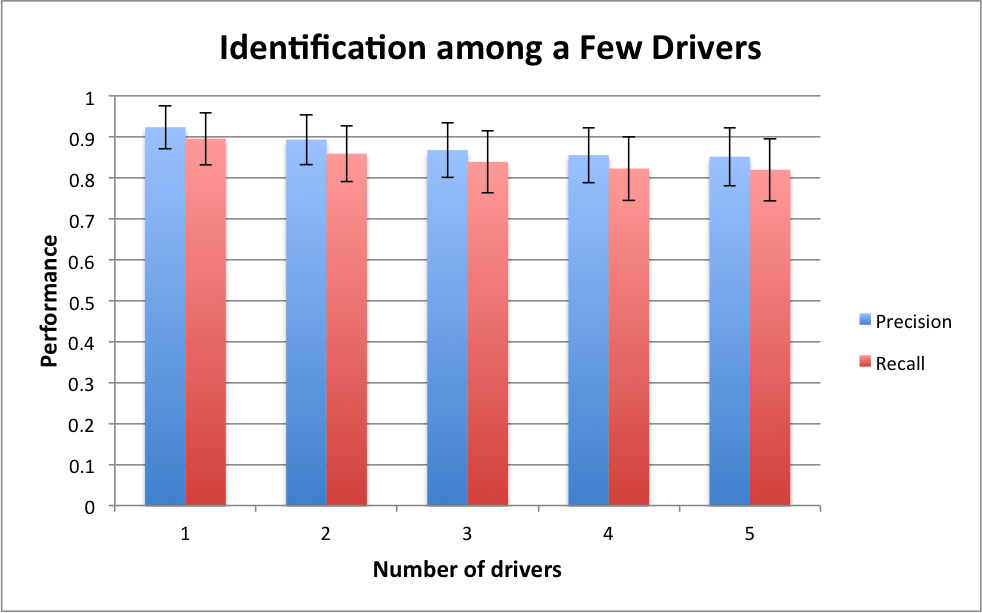
\includegraphics[width = 0.7\textwidth]{few_drivers.png}
\caption{Caption}
\label{fig:few}
\end{figure}


%cite statistics
%Statistics show that in most countries, the average household does not exceed 6 people. 

\subsection{Trip Matching}

\section{Discussion}
%What roadblocks did you encounter and how did you overcome them?
%no trip explicit matching in machine learning
%55 fake trips on average
\subsection{Obstacles}

The false trips added to each driver's data presented a major challenge. These false trips represent false data samples to be labeled as positive in the data, which can lower the performance of the classifier.

Initially, we assumed that only a small number false trips were added to each driver's data, but after carrying out several experiments, we suspected that the number of false trips might be larger than expected. To get a sense of the extent to which this addition of false trips might have affected the performance of our models, we found an estimate of the number of false trips for each driver. We downloaded the solution of the team which won second place in Kaggle's competition, which had received a score of 0.97; we then used their code to compute the probability that a given trip was made by the driver, whose data it appears in. We used this list to estimate that, on average 55.48 trips were added per driver with a standard deviation of 18.13; the minimum number of such trips was 15 and the maximum was 144. Thus, we can observe that the number of false trips often constitutes a non-trivial portion of a driver's data, which can have significant performance implications. 

\subsection{Future Directions}
We hope to find another similar dataset which does not contain false trips and use it to test the reliability of our model. 

%Incorporate trip matching into the classification?


\section{Conclusion}

\newpage
\nocite{*}
\bibliographystyle{plain}
\bibliography{biblio}


\section*{Appendix}
\subsection*{Who did what}

\end{document}
